\documentclass{acm_proc_article-sp}
%\documentclass{sig-alternate}
\usepackage{stmaryrd,amsmath,amssymb,newlfont,graphicx,verbatim}
\usepackage[ruled,lined,boxed,commentsnumbered,linesnumbered]{algorithm2e}
\usepackage{subfigure,url}
\usepackage{fancyvrb}


%\newtheorem{notation}[theorem]{Notation}

\newcounter{thedef} \setcounter{thedef}{1}
\newenvironment{definition}[1][]{\medskip\noindent {\textbf{Definition
  \arabic{thedef} #1} \stepcounter{thedef} \rm}}{\medskip}

\newcounter{theass} \setcounter{theass}{1}
\newenvironment{assumption}[1][]{\medskip\noindent {\textbf{Assumption
  \arabic{theass} #1} \stepcounter{theass} \rm}}{\medskip}

\newcounter{theeg} \setcounter{theeg}{1}
\newenvironment{example}[1][]{\medskip\noindent {\textbf{Example
  \arabic{theeg} #1} \stepcounter{theeg} \rm}{\medskip}}



\newcommand{\dom}{\mathrm{dom}}
\newcommand{\len}{\mathit{len}}
\newcommand{\poly}{\mathsf{poly}}
\newcommand{\flow}{\mathsf{flow}}
\newcommand{\jump}{\mathsf{jump}}
\newcommand{\inv}{\mathsf{inv}}
\newcommand{\init}{\mathsf{init}}
\newcommand{\guard}{\mathsf{guard}}
\newcommand{\reset}{\mathsf{reset}}
\newcommand{\reach}{\mathsf{Reach}}
\newcommand{\goal}{\mathsf{goal}}
\newcommand{\safe}{\mathsf{safe}}
\newcommand{\p}{\mathsf{P}}
\newcommand{\np}{\mathsf{NP}}
\newcommand{\R}{\mathbb{R}}
\newcommand{\lrf}{\mathcal{L}_{\mathbb{R}_{\mathcal{F}}}}
\newcommand{\citep}{\cite}

\newcommand{\hide}[1]{}
\newcommand{\eg}{{\em e.g.}}
\newcommand{\ie}{{\em i.e.}}
\newcommand{\enforce}{\mathsf{enforce}}




\begin{document}
\conferenceinfo{HSCC}{'15 Seattle, Washington, USA}


% a specific title
%\title{Identifying Personalized Hormone Therapy Schedules for Prostate Cancer Through Delta-Reachability Analysis
% a general title 
\title{Towards Personalized Cancer Therapy Using Delta-Reachability Analysis
\titlenote{This work has been partially supported by award N00014-13-1-0090 of the US Office of Naval Research and award CNS0926181 of the National Science foundation (NSF).}}

% alternative titles:
% Identifiying Optimized Intermittent Androgen Suppression Therapy Schedules for Prostate Cancer Using $\delta$-Decisions 
% Hybrid Modeling of Prostate Cancer Progression Reveals Optimized Angrogen Ablation Therapy Schedules
% Delta-Decision Based Analysis of a Hybrid Model for Prostate Cancer Progression

\numberofauthors{6} 
\author{
% 1st. author
\alignauthor
Bing Liu\\
       \affaddr{School of Medicine}\\
       \affaddr{University of Pittsburgh}\\
       \affaddr{Pittsburgh, PA, USA}\\
       \email{liubing@pitt.edu}
% 2nd. author
\alignauthor
Soonho Kong\\
       \affaddr{Computer Science Dept.}\\
       \affaddr{Carnegie Mellon University}\\
       \affaddr{Pittsburgh, PA, USA}\\
       \email{soonhok@cs.cmu.edu}
% 3rd. author
\alignauthor 
Sicun Gao\\
       \affaddr{CSAIL}\\
       \affaddr{MIT}\\
       \affaddr{Cambridge, MA, USA}\\
       \email{sicung@csail.mit.edu}
\and  % use '\and' if you need 'another row' of author names
% 4th. author
\alignauthor 
Paolo Zuliani\\
       \affaddr{School of Computer Science}\\
       \affaddr{Newcastle University}\\
       \affaddr{Newcastle, UK}\\
       \email{paolo.zuliani@ncl.ac.uk}
% 5th. author
\alignauthor 
Edmund M. Clarke\\
       \affaddr{Computer Science Dept.}\\
       \affaddr{Carnegie Mellon University}\\
       \affaddr{Pittsburgh, PA, USA}\\
       \email{emc@cs.cmu.edu}
}

\date{20 October 2014}


\maketitle

\begin{abstract}
Recent clinical studies suggest that the efficacy of hormone therapy for prostate cancer depends on the characteristics of individual patients. In this paper, we develop a computational framework for identifying patient-specific androgen ablation therapy schedules for postponing the potential cancer relapse. We model the population dynamics of heterogeneous prostate cancer cells in response to androgen suppression as a nonlinear hybrid automaton. We estimate personalized kinetic parameters to characterize patients and employ delta-reachability analysis to predict patient-specific therapeutic strategies. The results show that our methods are promising and may lead to a prognostic tool for personalized cancer therapy.
\end{abstract}


% Meta info
% [todo]

\category{D.2.4}{Software Engineering}{Software/Program Verification}[Model checking]
\category{J.3}{Life and Medical Sciences}{Biology and genetics}

\terms{Theory\\ Verification}

\keywords{hybrid systems, delta-reachability, systems biology, prostate cancer, personalized therapy}


\section{Introduction}\label{sec:intro}

% Need a paragrapgh or two to explain why the tool is interesting and
% significant should be provided.

\dReach{} is a bounded reachability analysis tool for hybrid systems.
It encodes bounded reachability problems of hybrid systems as
first-order formulas over the real numbers, and solves them using
$\delta$-decision procedures in the SMT solver
\dReal{}~\cite{DBLP:conf/cade/GaoKC13}. \dReach{} is able to handle a
wide range of highly nonlinear hybrid systems~\cite{CMSB14,DBLP:conf/fmcad/GaoKC13,DBLP:conf/hybrid/KapinskiDSA14,6868816}.
Figure~\ref{fig:prostate-example} highlights some of its features: on
the left is an example of some nonlinear dynamics that \dReach{} can
handle, and on the right a visualized counterexample generated by
\dReach{} on this model.
\begin{figure}[!h]
  \subfloat[An example of nonlinear hybrid system model: off-treatment
  mode of the prostate cancer treatment model~\cite{CMSB14}\label{subfig-1:prostate}]{
    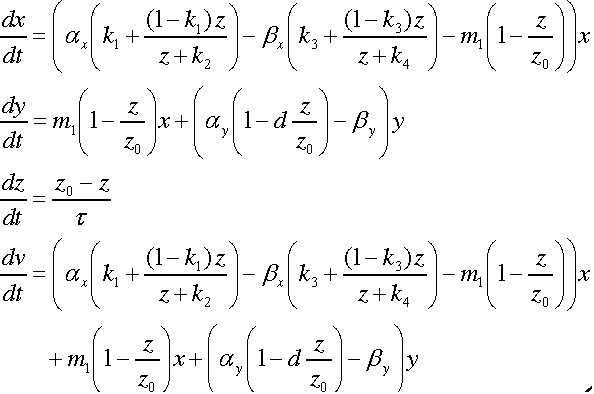
\includegraphics[width=0.45\textwidth]{images/prostatebw-mode2.pdf}
  }
  \hfill
  \subfloat[Visualization of a generated counterexample. Change in the shade of colors represents discrete mode changes.]{%
    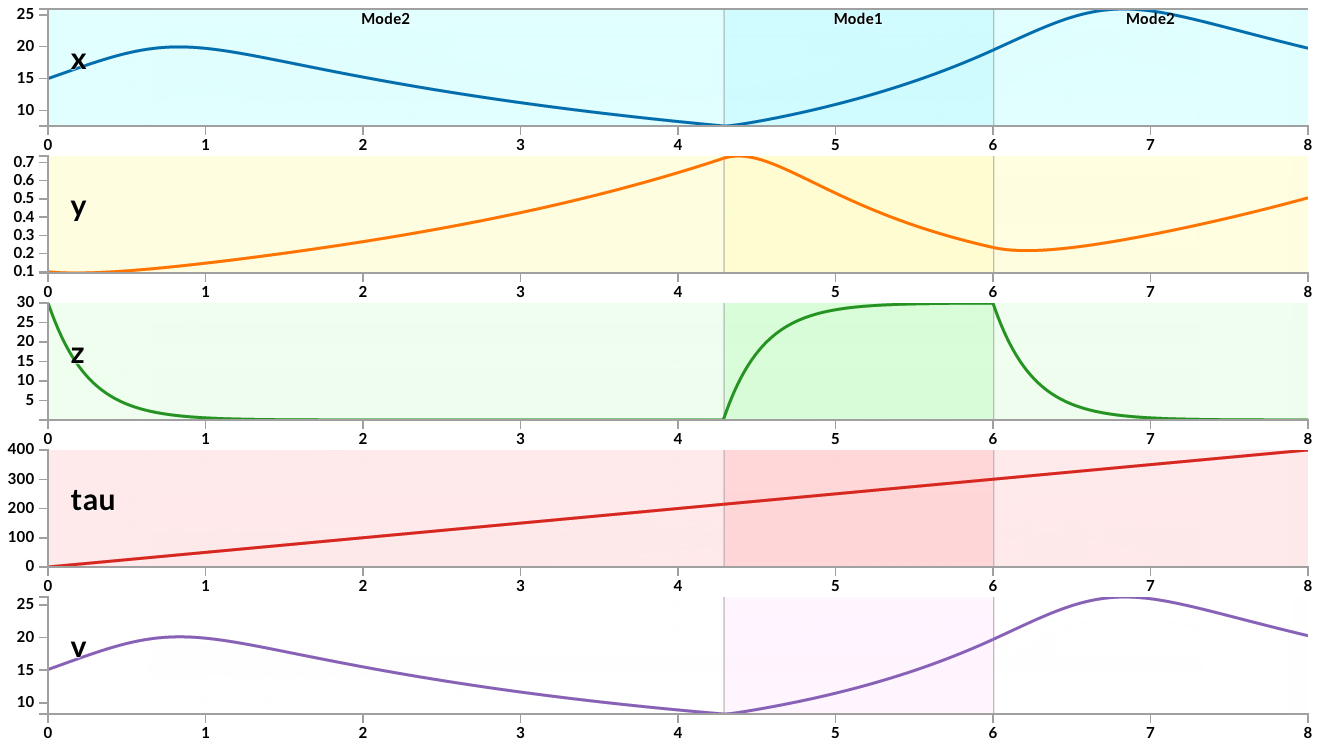
\includegraphics[width=0.48\textwidth]{images/prostate}
  }
  \caption{An example of nonlinear dynamics and counterexample-generation.}
  \label{fig:prostate-example}
\end{figure}

It is well-known that the standard bounded reachability problems for
simple hybrid systems are already highly
undecidable~\cite{DBLP:conf/hybrid/AlurCHH92}.
Instead, we work in the framework of $\delta$-reachability of hybrid systems~\cite{DBLP:journals/corr/GaoKCC14}.
Here $\delta$ is an arbitrary positive rational number, provided by the user to
specify the bound on numerical errors that can be tolerated in the analysis.
For a hybrid system $H$ and an unsafe region $\unsafe$ (both encoded as logic formulas),
the $\delta$-reachability problem asks for one of the following answers:
\begin{itemize}
        \item {\sf safe}: $H$ cannot reach $\unsafe$.
        \item {\sf $\delta$-unsafe}: $H^{\delta}$ can reach $\unsafe^{\delta}$.
\end{itemize}
Here, $H^{\delta}$ and $\unsafe^{\delta}$ encode ($\delta$-bounded) overapproximations
of $H$ and $\unsafe$, defined explicitly as their syntactic variants.%(See Section~\ref{sec:delta-reachability} in the Appendix.)
It is important to note that the definition makes the answers no weaker than standard reachability:
When {\sf safe} is the answer, we know for certain that $H$ does not reach
the unsafe region (no $\delta$ is involved); when {\sf $\delta$-unsafe} is the answer,
we know that there exists some $\delta$-bounded perturbation of the system that can render it unsafe.
Since $\delta$ can be chosen to be very small, {\sf$\delta$-unsafe} answers in fact
discover robustness problem in the system, which should be regarded as unsafe indeed.
We have proved that bounded $\delta$-reachabilty is decidable for a wide range
of nonlinear hybrid systems, even with reasonable complexity bounds~\cite{DBLP:journals/corr/GaoKCC14}.
This framework provides the formal correctness guarantees of \dReach{}.

Apart from solving $\delta$-reachability, the following key features of \dReach{}
distinguish it from other existing tools in this
domain~\cite{DBLP:journals/jlp/FranzleTE10,DBLP:conf/cav/FrehseGDCRLRGDM11,DBLP:journals/tac/AlthoffK14,DBLP:conf/hybrid/Frehse05,DBLP:conf/icons/HerdeEFT08,DBLP:conf/rtss/ChenAS12,DBLP:conf/aaai/CimattiMT12}.
%insert explanations for each item.
\begin{enumerate}
\item Expressiveness. \dReach{} allows the user to describe hybrid
  systems using first-order logic formulas over real numbers with a
  wide range of nonlinear functions. This allows the user to specify
  the continuous flows using highly nonlinear differential equations,
  and the jump and reset conditions with complex Boolean combinations
  of nonlinear constraints. \dReach{} also faithfully translates mode
  invariants into $\exists\forall$ logic formulas, which can be
  directly solved under certain restrictions on the invariants.
\item Property-guided search. \dReach{} maintains logical encodings
  (the same approach as~\cite{DBLP:conf/aaai/CimattiMT12}), whose size
  is linear in the size of the inputs, of the reachable states of a
  hybrid system~\cite{DBLP:journals/corr/GaoKCC14}. The tool searches
  for concrete counterexamples to falsify the reachability properties,
  instead of overapproximating the full reachable states. This avoids
  the usual state explosion problem in reachable set computation,
  because the full set of states does not need to be explicitly
  stored. This change is analogous to the difference between SAT-based
  model checking and BDD-based symbolic model checking.
\item Tight integration of symbolic reasoning and numerical solving.
  \dReach{} delegates the reasoning on discrete mode changes to SAT
  solvers, and uses numerical constraint solving to handle nonlinear
  dynamics. As a result, it can combine the full power of both
  symbolic reasoning and numerical analysis algorithms. In particular,
  all existing tools for reachable set computation can be easily
  plugged-in as engines for solving the continuous part of the
  dynamics, while logic reasoning tools can overcome the difficulty in
  handling complex mode transitions.
\end{enumerate}
The paper is structured as follows. We describe the system architecture in Section 2,
and give some details about the logical encoding in the tool in Section 3.
We then explain the input format and usage in Section 4. %More details and examples are given in the Appendix.

%Realistic hybrid systems involves nonlinear ODEs with transcendental
%functions. \dReach{} allows users to specify a hybrid system in a
%nonlinear signature as it is without linearizing or overapproximating
%it. Users can provide the tool with a numerical error bound $\delta$,
%a bounded time horizon $[0, T]$, and a maximum number of mode switches
%$k$ for the analysis. As a result of analysis, \dReach{} will return
%either \textbf{$\delta$-sat} with a concrete counterexample, or
%\textbf{unsat} which does not involve numerical errors. We also
%provide a visualization for the $\delta$-sat case to help
%understand the analysis result.

% TODO: Need to differentiate this paper from FMCAD paper
%  - FMCAD: underlying solving techniques for SMT with ODEs
%  - TACAS: tool, encoding, using solver...

%%% Local Variables:
%%% mode: latex
%%% TeX-master: "main"
%%% End:

\section{Model}

The model has two modes which are shown in Figure \ref{pmodel}. $x(t)$, $y(t)$, and $z(t)$ represent the population of AD cells, the population of AI cells, and the serum androgen concentration, respectively. The growth dynamics of AD and AI cells are governed by their proliferation rate, apoptosis rate and mutation rate from AD to AI phenotype, depending on androgen concentration $z(t)$. The PSA level $v$ (ng ml$^{-1}$) is defined as $v(t)=x(t)+y(t)$. The treatment is suspended or restarted according to the value of $v$ and ${dv}/{dt}$. In mode $2$ (off-treatment), the androgen concentration is maintained at the normal level $z_0$ by homeostasis. In mode $1$ (on-treatment), the androgen is cleared at a rate $1/\tau$. Table \ref{prostate} lists the values of model parameters.

\begin{figure}[htb]
\centering
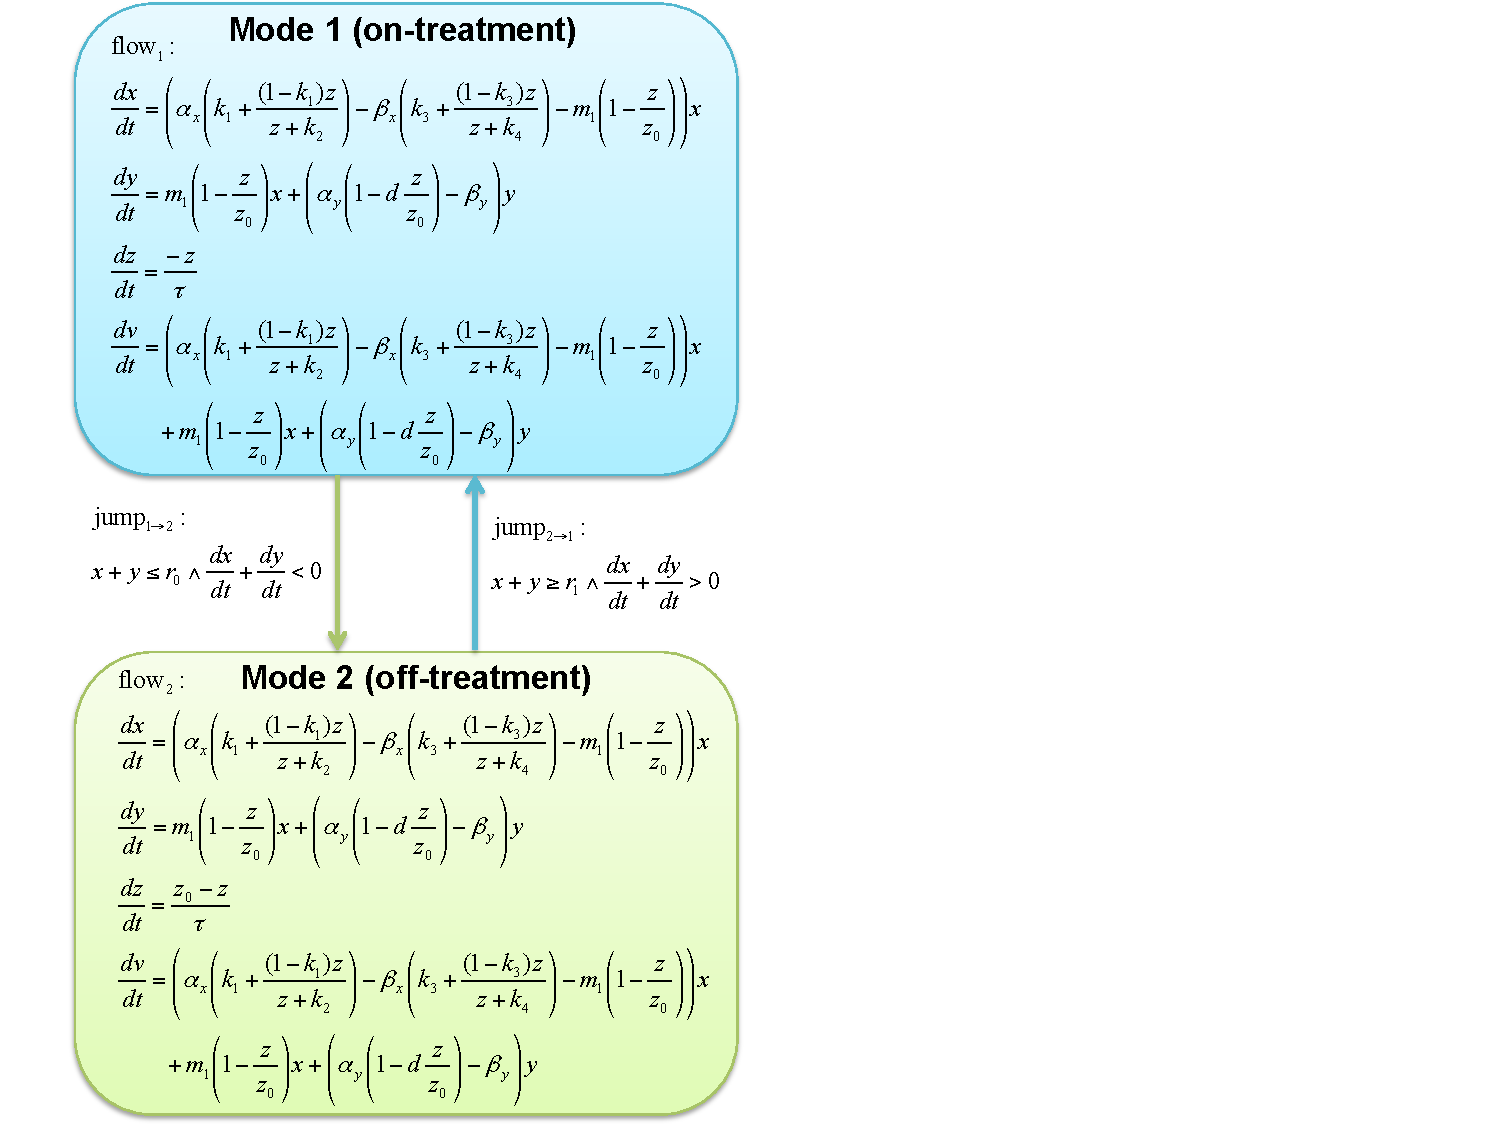
\includegraphics[scale=0.6]{fig-prostate}
\caption{The prostate cancer treatment model.}
\label{pmodel}
 %\vspace{-0.7cm}
\end{figure}

\begin{table}[h]
\caption{Prostate cancer model parameter values\label{prostate}}
\centering
\begin{tabular}{c|c|c}
\hline
Parameter  & Bone metastasis & Lymph node metastasis  \\\hline
$\alpha_x$ & 0.0204 d$^{-1}$ & 0.0168 d$^{-1}$  \\
$\alpha_y$ & 0.0242 d$^{-1}$ & 0.0277 d$^{-1}$  \\
$\beta_x$  & 0.0076 d$^{-1}$ & 0.0085 d$^{-1}$  \\
$\beta_y$  & 0.0168 d$^{-1}$ & 0.0222 d$^{-1}$  \\
$k_1$     & 0.0 nM & 0.0 nM \\
$k_2$     & 2.0 & 2.0  \\
$k_3$     & 8.0 nM & 8.0 nM \\
$k_4$     & 0.5 & 0.5  \\
$m_1$     & 0.00005 d$^{-1}$ & 0.00005 d$^{-1}$  \\
$z_0$     & 20.0 nM & 20.0 nM  \\
$\tau$     & 62.5 d & 62.5 d \\
\hline
\end{tabular}
 %\vspace{-0.7cm}
\end{table}

\section{$\delta$-Decisions for Hybrid Models}
We encode reachability problems of hybrid automata using a first-order language $\lrf$ over the reals, 
which allows the use of a wide range of real functions including nonlinear ODEs. 
We then use $\delta$-complete decision procedures to find solutions to these formulas to synthesize 
parameters. 

\begin{definition}[$\lrf$-Formulas]
Let $\mathcal{F}$ be a collection of computable real functions. We define:
\begin{align*}
t& := x \; | \; f(t(\vec x)), \mbox{ where }f\in \mathcal{F} \mbox{ (constants are 0-ary functions)};\\
\varphi& := t(\vec x)> 0 \; | \; t(\vec x)\geq 0 \; | \; \varphi\wedge\varphi
\; | \; \varphi\vee\varphi \; | \; \exists x_i\varphi \; |\; \forall x_i\varphi.
\end{align*}
\end{definition}
By computable real function we mean Type 2 computable, which informally requires that a (real) 
function can be algorithmically evaluated with arbitrary accuracy. Since in general 
$\lrf$ formulas are undecidable, the decision problem needs to be relaxed. In particular, for 
any $\lrf$ formula $\phi$ and any rational $\delta >0$ one can obtain a $\delta$-weakening 
formula $\phi^\delta$ from $\phi$ by substituting the atoms $t > 0$ with $t > -\delta$ (and
similarly for $t \geq 0$). Obviously, $\phi$ implies $\phi^\delta$, but not the {\em vice versa}.
Now, the $\delta$-decision problem is deciding correctly whether:
\begin{itemize}
	\item $\phi$ is false ($\mathsf{unsat}$);
	\item $\phi^\delta$ is true ($\delta$-$\mathsf{sat}$).
\end{itemize}
If both cases are true, then either decision is correct. In previous work~\cite{gao12a,gao12b,gao13}
we presented algorithms ($\delta$-{\em complete} decision procedures) for solving $\delta$-decision 
problems for $\lrf$ and for ODEs. These algorithms have been implemented in the dReal 
toolset \cite{dreal}. More details on $\delta$-decision problems are in Appendix. %(\verb#http://www.cs.cmu.edu/~liubing/cmsb14/#). 

Now we state the encoding for hybrid models. Recall that hybrid automata generalize finite-state
automata by permitting continuous-time evolution (or {\em flow}) in each discrete state (or {\em mode}). 
Also, in each mode an {\em invariant} must be satisfied by the flow, and mode switches are controlled
by {\em jump} conditions.
\begin{definition}[$\lrf$-Representations of Hybrid Automata]\label{lrf-definition}
A hybrid automaton in $\lrf$-representation is a tuple
\begin{multline*}
H = \langle X, Q, \{{\flow}_q(\vec x, \vec y, t): q\in Q\},\{\inv_q(\vec x): q\in Q\},\\
\{\jump_{q\rightarrow q'}(\vec x, \vec y): q,q'\in Q\},\{\init_q(\vec x): q\in Q\}\rangle
\end{multline*}
where $X\subseteq \mathbb{R}^n$ for some $n\in \mathbb{N}$, $Q=\{q_1,...,q_m\}$ is a finite set of modes, and the other components are finite sets of quantifier-free $\lrf$-formulas.
\end{definition}
\begin{example}[Nonlinear Bouncing Ball]
The bouncing ball is a standard hybrid system model. It can be $\lrf$-represented in the following way:
\begin{itemize}
\item $X = \mathbb{R}^2$ and $Q = \{q_u, q_d\}$. We use $q_u$ to represent bounce-back mode and $q_d$ the falling mode.
\item $\flow = \{\flow_{q_u}(x_0, v_0, x_t, v_t, t), \flow_{q_d}(x_0, v_0, x_t, v_t, t)\}$. We use $x$ to denote the height of the ball and $v$ its velocity. Instead of using time derivatives, we can directly write the flows as integrals over time, using $\lrf$-formulas:
\begin{itemize}
\item $\flow_{q_u}(x_0, v_0, x_t, v_t, t)$ defines the dynamics in the bounce-back phase:
$$(x_t = x_0 + \int_0^{t} v(s) ds) \wedge (v_t = v_0 + \int_0^t g(1-\beta v(s)^2) ds)$$
\item $\flow_{q_d}(x_0, v_0, x_t, v_t, t)$ defines the dynamics in the falling phase:
$$(x_t = x_0 + \int_0^{t} v(s) ds) \wedge (v_t = v_0 + \int_0^t g(1+\beta v(s)^2) ds)$$
\end{itemize}where
$\beta$ is a constant. Again, note that the integration terms define Type 2 computable functions.
\item $\jump = \{\jump_{q_u \rightarrow q_d} (x, v, x', v'), \jump_{q_d \rightarrow q_u} (x, v, x', v')\}$ where
\begin{itemize}
\item $\jump_{q_u \rightarrow q_d} (x, v, x', v')$ is $(v= 0 \wedge x' = x \wedge v' = v)$.
\item $\jump_{q_d \rightarrow q_u} (x, v, x', v')$ is $(x= 0 \wedge v' = \alpha v\wedge x'=x)$,  for some constant $\alpha$.
\end{itemize}
\item $\init_{q_d}$ is $(x=10 \wedge v=0)$ and $\init_{q_u}$ is $\bot$.
\item $\inv_{q_d}$ is $(x>=0 \wedge v>=0)$ and $\inv_{q_u}$ is $(x>=0 \wedge v<=0)$.
\end{itemize}
\end{example}

We now show the encoding of bounded reachability, which is used for encoding the parameter synthesis
problem. We want to decide whether a given 
hybrid system reaches a particular region of its state space after following a (bounded) number
of discrete transitions, \ie, jumps. First, we need to define auxiliary formulas used
for ensuring that a particular mode is picked at a certain step.
\begin{definition}
Let $Q = \{q_1,...,q_m\}$ be a set of modes. For any $q\in Q$, and $i\in\mathbb{N}$, use  $b_{q}^i$ to represent a Boolean variable. We now define
$$\enforce_Q(q,i) = b^i_{q} \wedge \bigwedge_{p\in Q\setminus\{q\}}\neg b^{i}_{p}$$
$$\enforce_Q(q, q',i) = b^{i}_{q}\wedge \neg b^{i+1}_{q'} \wedge \bigwedge_{p\in Q\setminus\{q\}} \neg b^i_{p} \wedge \bigwedge_{p'\in Q\setminus\{q'\}} \neg b^{i+1}_{p'}$$
We omit the subscript $Q$ when the context is clear.\end{definition}

We can now define the following formula that checks whether a {\em goal} region of the automaton
state space is reachable after exactly $k$ discrete transitions. We first state 
the simpler case of a hybrid system without invariants.
\begin{definition}[$k$-Step Reachability, Invariant-Free Case]
Suppose $H$ is an invariant-free hybrid automaton, $U$ a subset of its state space represented by $\goal$,
and $M>0$. The formula $\reach_{H,U}(k,M)$ is defined as:
\begin{eqnarray*}
%\reach^{k,M}(H,U) &:=&
& &\exists^X \vec x_{0} \exists^X\vec x_{0}^t\cdots \exists^X \vec x_{k}\exists^X\vec x_{k}^t\exists^{[0,M]}t_0\cdots \exists^{[0,M]}t_k.\\
& &\bigvee_{q\in Q} \Big(\init_{q}(\vec x_{0})\wedge \flow_{q}(\vec x_{0}, \vec x_{0}^t, t_0)\wedge \enforce(q,0)\Big)\\%\wedge (b_{q_i}\wedge \bigwedge_{q\neq q_i} \neg b_{q})
\wedge & & \bigwedge_{i=0}^{k-1}\bigg( \bigvee_{q, q'\in Q} \Big(\jump_{q\rightarrow q'}(\vec x_{i}^t, \vec x_{i+1})\wedge \enforce(q,q',i)\\
& & \hspace{4.5cm}\wedge\flow_{q'}(\vec x_{i+1}, \vec x_{i+1}^t, t_{i+1})\wedge \enforce(q',i+1)\Big)\bigg)\\
\wedge & &\bigvee_{q\in Q} (\goal_q(\vec x_{k}^t)\wedge \enforce(q,k))
\end{eqnarray*}
where $\exists^X x$ is a shorthand for $\exists x\in X$.
\end{definition}
Intuitively, the trajectories start with some initial state satisfying $\init_q(\vec x_{0})$ for some $q$. 
Then, in each step the trajectory follows $\flow_q(\vec x_{i}, \vec x_{i}^t, t)$ and makes a continuous flow from $\vec x_i$ to $\vec x_i^t$ after time $t$. When the automaton makes a $\jump$ from mode $q'$ to $q$, it resets variables following $\jump_{q'\rightarrow q}(\vec x_{k}^t, \vec x_{k+1})$. The auxiliary $\enforce$ formulas ensure that picking $\jump_{q\rightarrow q'}$ in the $i$-the step enforces picking $\flow_q'$ in the $(i+1)$-th step.

When the invariants are not trivial, we need to ensure that for all the time points along a continuous flow, the invariant condition holds. We need to universally quantify over time, and the encoding is as follows:
\begin{definition}[$k$-Step Reachability, Nontrivial Invariant]\label{br2}
Suppose $H$ contains invariants, and $U$ is a subset of the state space represented by $\goal$. The $\lrf$-formula $\reach_{H,U}(k,M)$ is defined as:
\begin{eqnarray*}
& &\exists^X \vec x_{0} \exists^X\vec x_{0}^t\cdots \exists^X \vec x_{k}\exists^X\vec x_{k}^t \exists^{[0,M]}t_0\cdots \exists^{[0,M]}t_k.\\
& &\bigvee_{q\in Q} \Big(\init_{q}(\vec x_{0})\wedge \flow_{q}(\vec x_{0}, \vec x_{0}^t, t_0)\wedge \enforce(q,0)\\
& &\hspace{5cm} \wedge \forall^{[0,t_0]}t\forall^X\vec x\;(\flow_{q}(\vec x_{0}, \vec x, t)\rightarrow \inv_{q}(\vec x))\Big) \\
\wedge & &\bigwedge_{i=0}^{k-1}\bigg( \bigvee_{q, q'\in Q} \Big(\jump_{q\rightarrow q'}(\vec
x_{i}^t, \vec x_{i+1})\wedge \flow_{q'}(\vec x_{i+1}, \vec x_{i+1}^t, t_{i+1})\wedge \enforce(q,q',i)\\
& & \hspace{1.5cm}\wedge\enforce(q',i+1)\wedge \forall^{[0,t_{i+1}]}t\forall^X\vec x\;(\flow_{q'}(\vec x_{i+1}, \vec x,
t)\rightarrow \inv_{q'}(\vec x)) )\Big)\bigg)\\
\wedge & &\bigvee_{q\in Q} (\goal_q(\vec x_{k}^t)\wedge \enforce(q,k)).
\end{eqnarray*}
\end{definition}
The extra universal quantifier for each continuous flow expresses the requirement that for all the time points between the initial and ending time point ($t\in[0,t_i+1]$) in a flow, the continuous variables $\vec x$ must take values that satisfy the invariant conditions $\inv_q(\vec x)$.

\paragraph{Parameter Identification.}
The parameter identification problem we tackle is basically a $k$-step reachability question: Is there a parameter
combination for which the model reaches the goal region in $k$ steps? If none exists, then the model is 
{\em unfeasible}. Otherwise, a witness (\ie, a value for each parameter) is returned. Note that because we ask for
$\delta$-decisions, the returned witness might correspond to a {\em spurious} behavior of the system. The occurrence
of such behaviors can be controlled via the precision $\delta$, but in general cannot be eliminated. 
We have developed the dReach tool (\verb#http://dreal.cs.cmu.edu/dreach.html#) 
that automatically builds reachability formulas from a hybrid model and a goal 
description. Such formulas are then verified by our $\delta$-complete solver dReal \citep{dreal}.





\section{Case Study}
% PZ: I think the two sentences below should in 'Methods' section.
%We have developed an open-source tool dReach using OCaml to perform $\delta$-complete reachability 
%analysis for hybrid systems \cite{dreach}. dReach is built upon our SMT solver dReal \citep{dreal} 
%that implements a $\delta$-complete decision procedure. 

To exemplify different aspects of our parameter synthesis framework, we carried out a case study on
a model of the electrical dynamics of cardiac cells. All the experiments reported below were done 
using a machine with two Intel Xeon E5-2650 2.00GHz processors and 64GB RAM. The precision $\delta$
was set to $0.001$.

\begin{figure}[t]
\centering
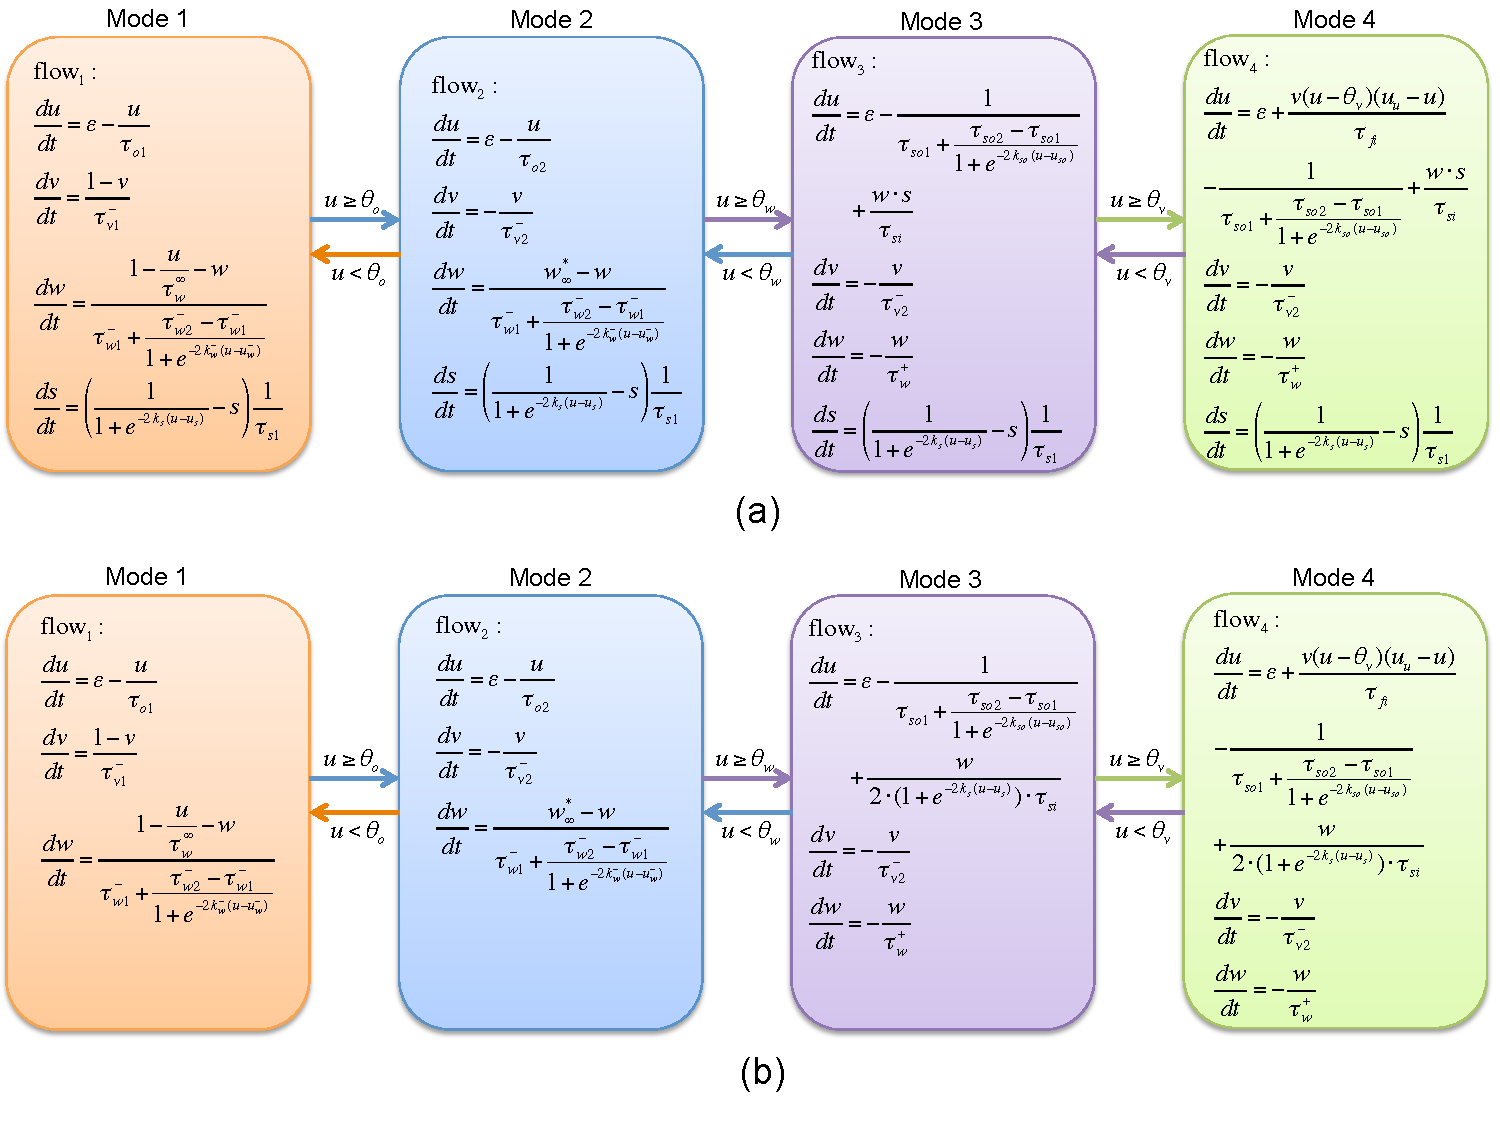
\includegraphics[scale=0.5]{fig-cardiac-new}
\caption{Hybrid models of cardiac cells. (a) BCF model. (b) FK model.}
\label{model}
 %\vspace{-0.7cm}
\end{figure}

\subsection{Hybrid models of cardiac cells}
The heart rhythm is enabled by the electrical activity of cardiac muscle cells, which make up the atria and ventricles. The electrical dynamics of cardiac cells is governed by the organized opening and closing of ion channel gates on the cell membrane. Improper functioning of the cardiac cell ionic channels can cause the cells to lose excitability, which disorders electric wave propagation and leads to cardiac abnormalities such as ventricular \textit{tachycardia} or \textit{fibrillation}. Hybrid automata models have been developed recently in order to understand the mechanisms of cardiac disorders, including the Fenton-Karma (FK) model \cite{fenton98} and the Bueno-Cherry-Fenton (BCF) model \cite{orovio08}. 

\paragraph{BCF Model.} 
In this model, the change of cells transmembrane potential $u$, in response to an external stimulus $\epsilon$ from neighboring cells, is regulated by a fast ion channel gate $v$ and two slow gates $w$ and $s$.
Figure \ref{model}(a) shows the four modes associated with the BCF model. In Mode $1$, gates $v$ and $w$ are open and gate $s$ is closed. The transmembrane potassium current causes the decay of $u$. The cell is resting and waiting for stimulation. We assume an external stimulus $\epsilon$ equals to $1$ which lasts for $1$ millisecond. The stimulation causes $u$ to increase, which may trigger $\jump_{1 \rightarrow 2}: u \geq \theta_o$. When this jump takes place, the system switches to Mode 2 and $v$ starts closing, and the decay rate of $u$ changes. The system will jump to Mode 3 if $u \geq \theta_w$. In Mode 3, $w$ is also closing; $u$ is governed by the potassium current and the calcium current. When $u \geq \theta_v$, Mode 4 can be reached, which signals a successful action potential (AP) initiation. In Mode 4, $u$ reaches its peak due to the fast opening of the sodium channel. The cardiac muscle contracts and $u$ starts decreasing. 

\paragraph{FK Model.} 
As shown in Figure \ref{model}(b), this model comprises the same four modes and equations of the BCF model, except that the current change induced by gate $s$ is reduced to an explicit term which is integrated
in the right-hand side of $du/dt$. Similarly to the BCF model, an AP can be successfully initiated when Mode 4 is reached. 

We specified both the BCF and the FK model using dReach's modeling language. Starting from the state ($u = 0$, $v = 1$, $w = 1$, $s = 0$) in Mode 1, we checked whether Mode 4 is reachable using the parameter values presented in \cite{orovio08}. This was true (\ie, dReach returned $\delta$-$\mathsf{sat}$) for both models. 
The simulation of a few witness trajectories are shown in Figure \ref{trace} (the stimulus $\epsilon$ was reset every $500$ milliseconds).


\begin{figure}[thb]
\centering
\subfigure[]{
  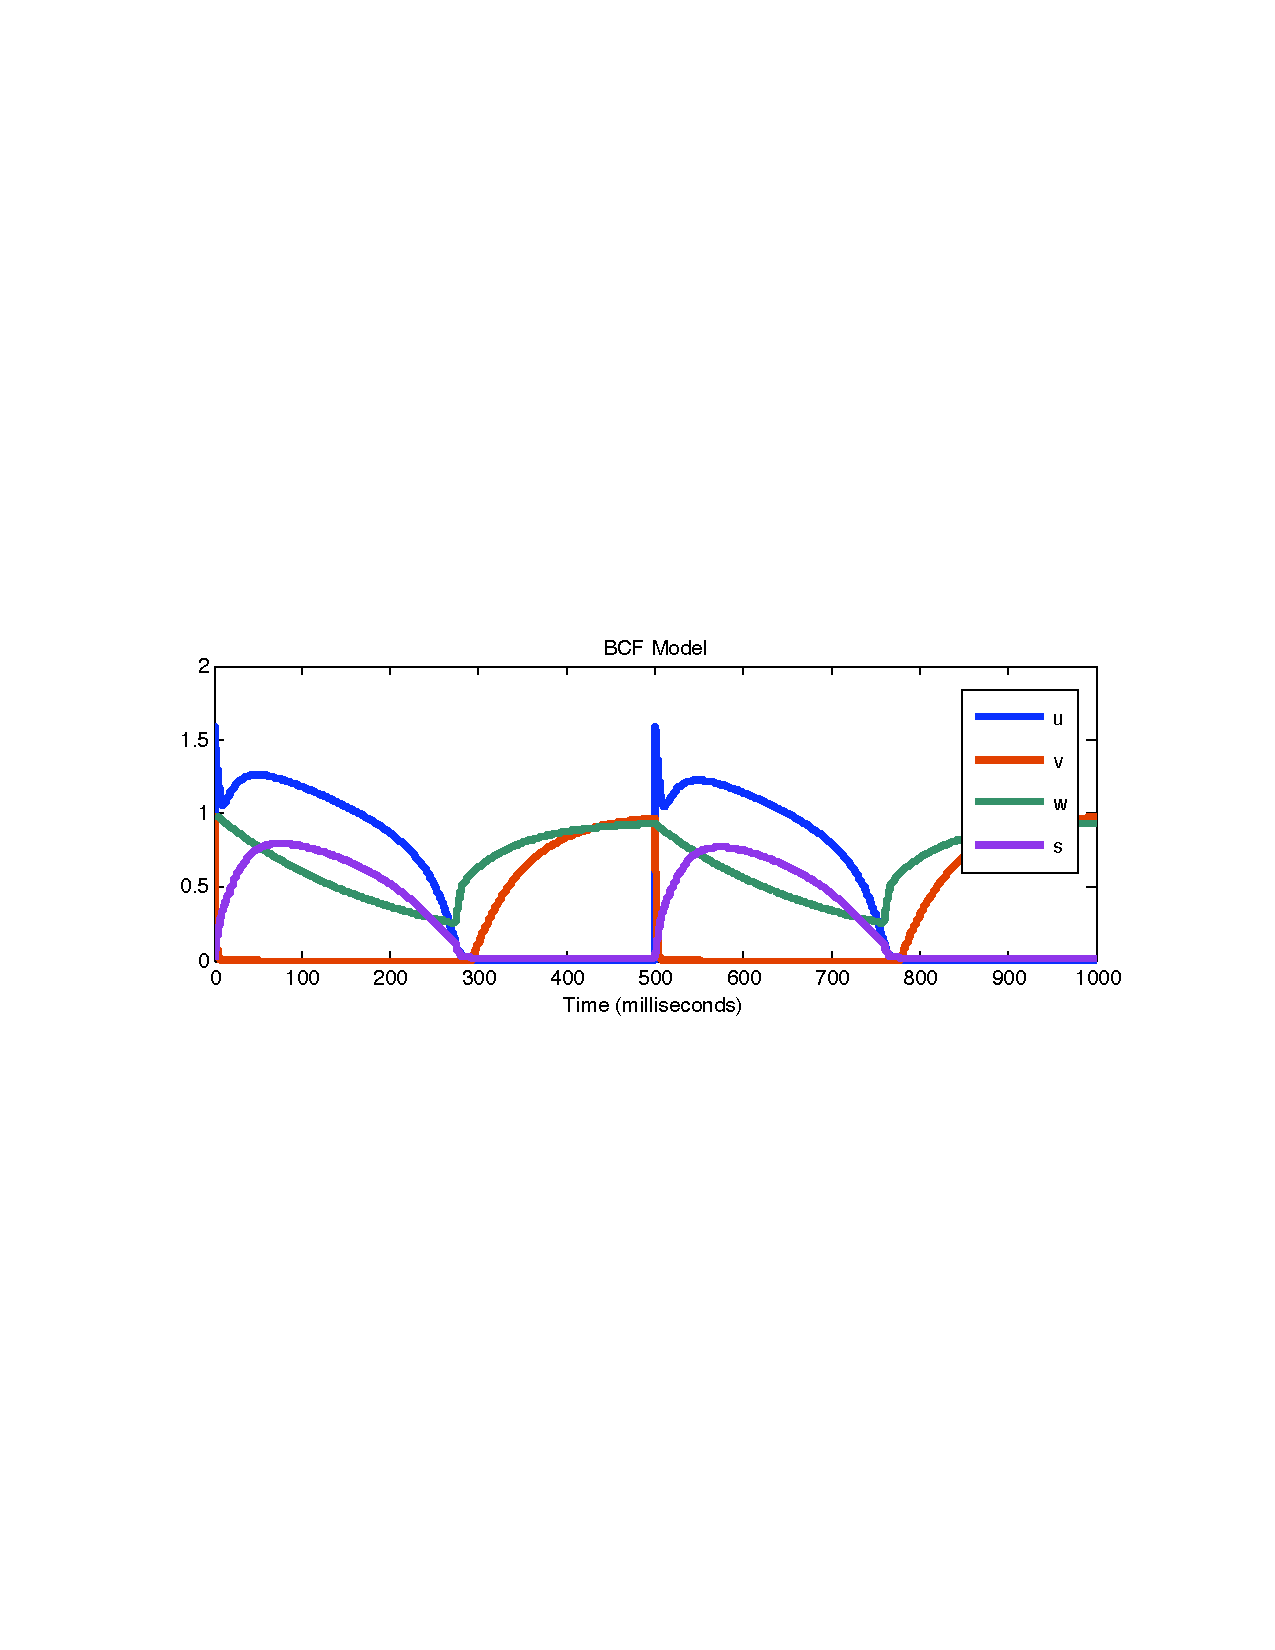
\includegraphics[width=8cm]{fig-bcf}
} 
\subfigure[]{
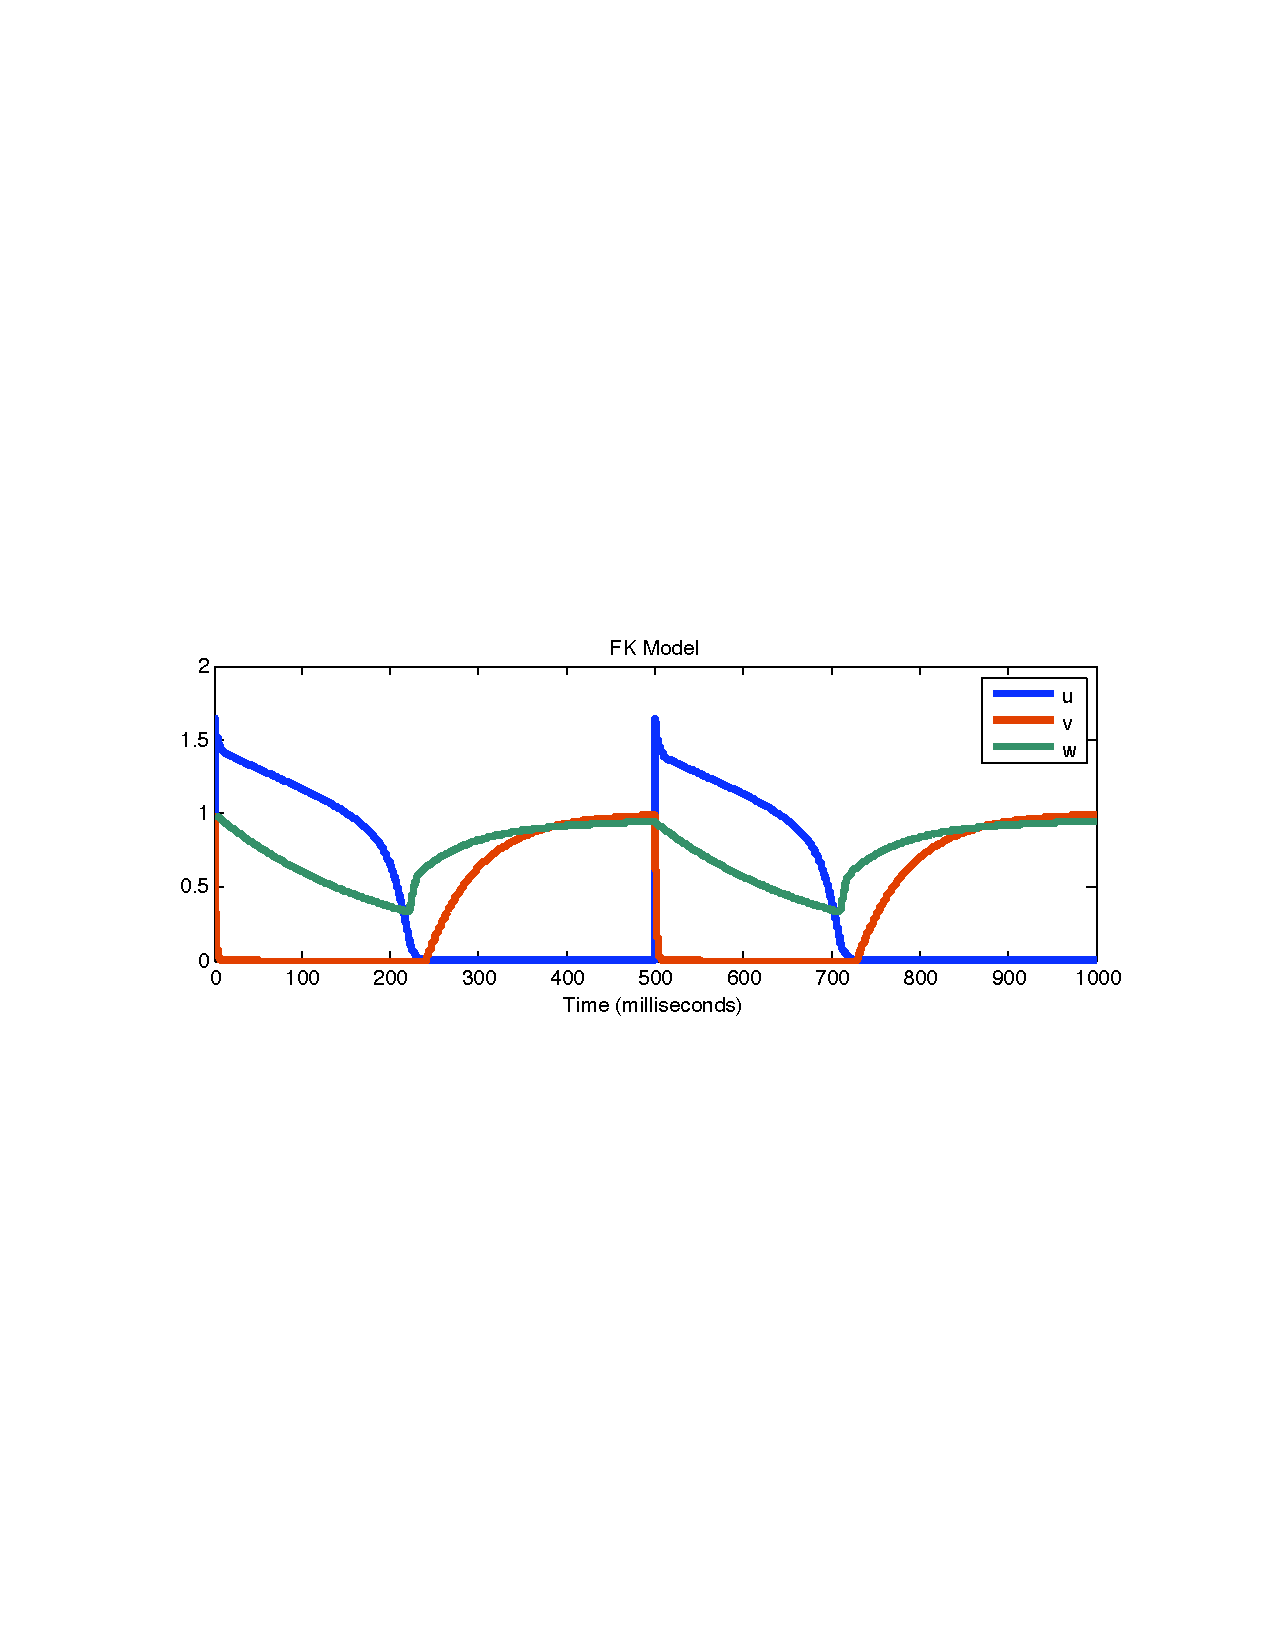
\includegraphics[width=8cm]{fig-fk}
}
\caption{The simulated time profile of BCF and FK.}
\label{trace}
 %\vspace{-0.7cm}
\end{figure}


\subsection{Model falsification}
Both the BCF and FK models were able to reproduce essential characteristics (\eg, steady-state action potential duration) observed in human ventricular cells \cite{fenton98,orovio08}. However, ventricular cells comprise three cell types, which possess different dynamical characteristics. For instance, Figure \ref{ap} shows that time courses of APs for epicardial and endocardial human ventricular cells have different morphologies \cite{nabauer96}. An important \textit{spike-and-dome} AP morphology can only be observed in epicardial cells but not endocardial cells. Hence, in a model-based study, one needs to identify cell-type-specific parameters to take account into cellular heterogeneity. The feasibility of this task will depend on the model of choice, as certain model would be impossible to reproduce a dynamical behavior no matter which parameter values are used. Here we illustrate that such models can be ruled out efficiently using our $\delta$-decision based parameter synthesis framework.

\paragraph{Robustness.} 
To ensure proper functioning of cardiac cells in noisy environments, an important property of the system is to filter out insignificant stimulation. Thus, we expected to see that APs could not be initiated for small $\epsilon$. Starting from the state ($u = 0$, $v = 1$, $w = 1$, $s = 0$, $\epsilon \in [0.0,0.25]$) in Mode 1, we checked the reachability of Mode 4. The $\mathsf{unsat}$ answer was returned by dReach for both the BCF and FK
model, showing that the models are robust to stimulation amplitude.

\begin{figure}[th]
\centering
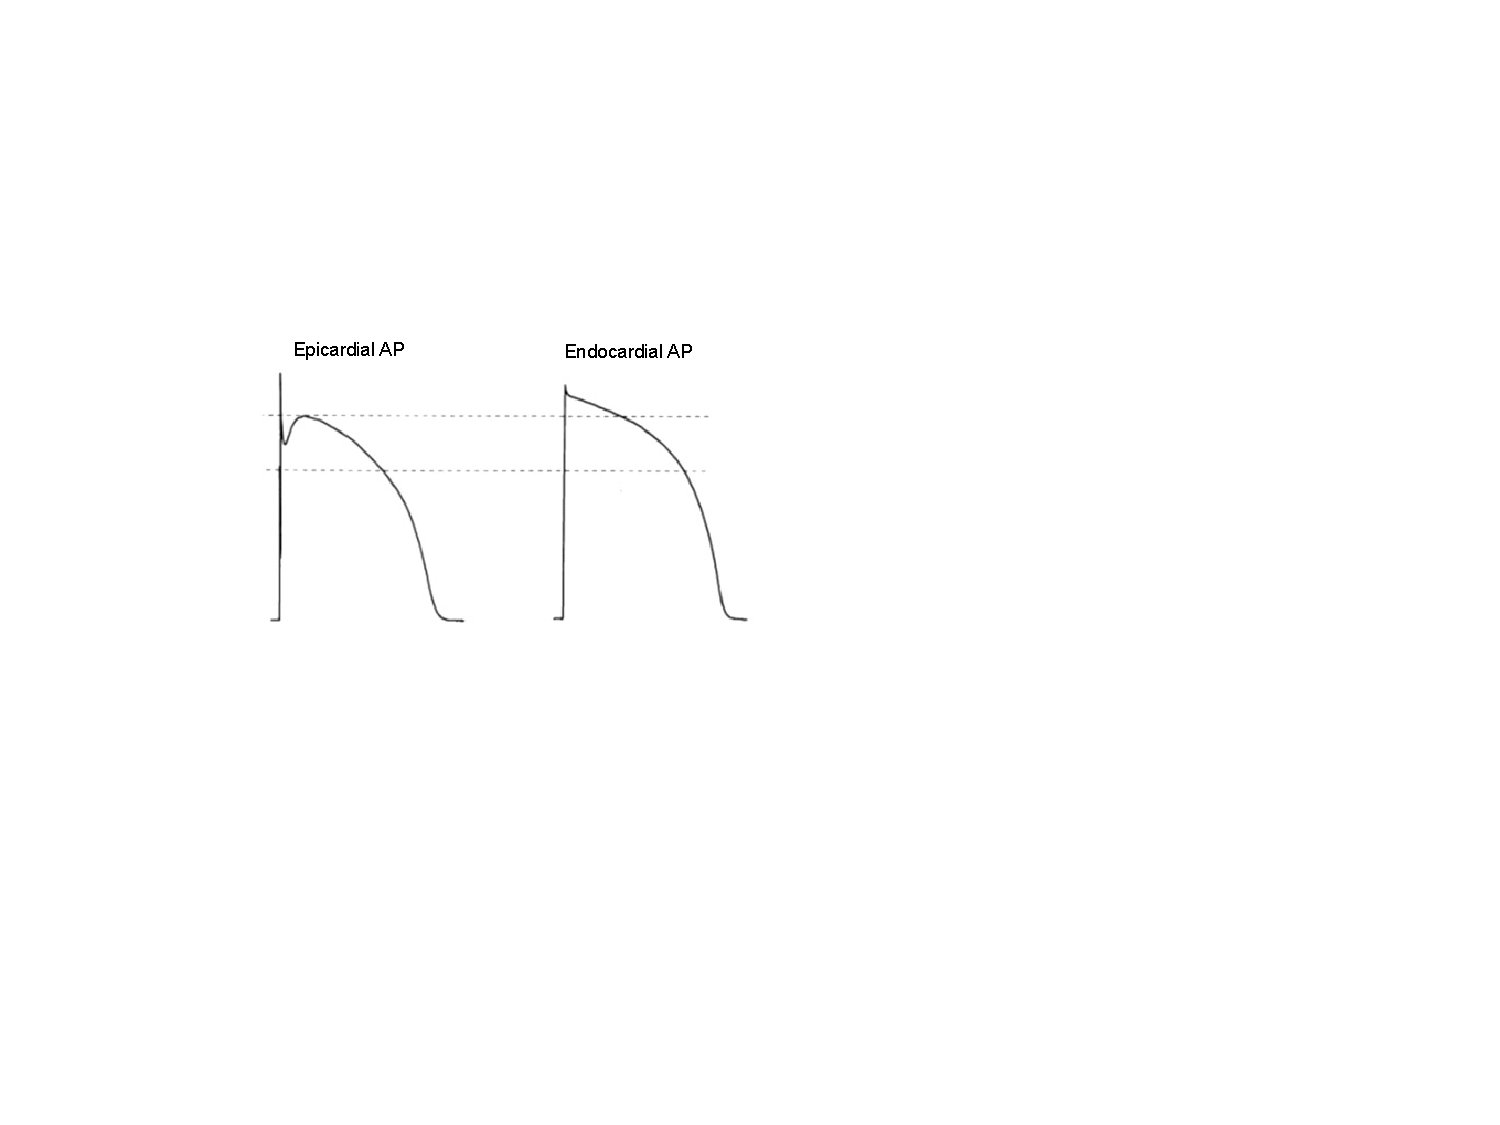
\includegraphics[scale=0.8]{fig-ap}
\caption{Experimental AP morphology \cite{nabauer96}.}
\label{ap}
 %\vspace{-0.7cm}
\end{figure}

\paragraph{AP morphology.}
Next we tested whether the models can reproduce the spike-and-dome AP morphology of epicardial cells. We introduced two auxiliary modes (Mode 5 and 6). The system will jump from Mode 4 to Mode 5 if $\tau \le 10$, and will jump from Mode 5 to Mode 6 if $\tau \le 30$. In Modes 5 and 6, we enforced invariants $1.0 \le u \le 1.15$ and $1.18 \le u \le 2.0$, respectively, to depict the spike-and-dome morphology observed experimentally \cite{nabauer96}. We then checked reachability of Mode 6, starting from Mode 1 in state ($u = 0$, $v = 1$, $w = 1$, $s = 0$, $\epsilon \in [0.9,1.1]$, $\tau_{si} \in [1,2]$, $u_s \in [0.5,2]$). The $\delta$-$\mathsf{sat}$ answer
was returned for BCF, while $\mathsf{unsat}$ was returned for FK, indicating that the FK model cannot reproduce spike-and-dome shapes using reasonable parameter values. Hence, FK is not suitable to study the dynamics of epicardial cells.

We remark that any $\mathsf{unsat}$ answer is guaranteed to be correct. This effectively
means that we proved that the FK model cannot reach Mode 6 for {\em any} starting state in the 
rectangle ($u = 0$, $v = 1$, $w = 1$, $s = 0$, $\epsilon \in [0.9,1.1]$, $\tau_{si} \in [1,2]$, 
$u_s \in [0.5,2]$). Sampling-based approaches cannot have the same level of certainty, while other
approaches cannot handle the complexity of the flows in the model.


\subsection{Parameter identification for cardiac disorders}

When the system cannot reach Mode 4, the cardiac cell loses excitability, which might lead to tachycardia or fibrillation. Starting with Mode 1, our next goal was to identify parameter ranges for which the system will never go into Mode 4. In what follows, we focused our study on the BCF model. 
Grosu {\em et al.}~\cite{grosu11} have tackled this parameter identification problem by linearizing the BCF model into a piecewise-multiaffine system (referred as MHA). With this simplification, parameter ranges could be identified using the Rovergene tool \cite{rovergene}. However, the BCF and MHA models have different sets of parameters. Here we aimed at identifying disease-related ranges of the original BCF parameters. It can be derived from the model equations that $\tau_{o1}$ and $\tau_{o2}$ govern the dynamics of $u$ in Mode 1 and Mode 2 respectively, and hence determine whether $\jump_{1\rightarrow 2}$ and  $\jump_{2\rightarrow 3}$ can be triggered. For $\tau_{o1}$, we performed a binary search in value domain $[0.0001,0.01]$ to obtain a threshold value $\theta_{o1}$ such that Mode 4 is unreachable if $\tau_{o1} \in (0, \theta_{o1})$ while Mode 4 is reachable if $\tau_{o1} =  \theta_{to1}$. Specifically, for each candidate value $\theta^i_{o1}$, we checked the reachability of Mode 4 with the initial state ($u = 0$, $v = 1$, $w = 1$, $s = 0$, $\theta_{o1} = \theta^i_{o1}$). We set the next candidate to be $(\theta^i_{o1} -\theta_{l})/2$ if $\mathsf{sat}$ was returned, or $(\theta_{r} - \theta^i_{o1})/2$ if $\mathsf{unsat}$ was returned, where $\theta_{l}$ is the largest $\mathsf{unsat}$ candidate and $\theta_{r}$ is the smallest $\mathsf{sat}$ candidate. 

In this manner, we identified $\theta_{o1}$ to be $0.006$, which suggest that when $\tau_{o1} \in (0, 0.006)$, the system will always stay in Mode 1. Similarly, we also obtained a threshold value of $0.13$ for $\tau_{o2}$, such that Mode 3 cannot be reached when $\tau_{o2} \in (0, 0.13)$. Furthermore, whether the system can jump from Mode 3 to Mode 4 depends on the interplay between $\tau_{so1}$ and $\tau_{so2}$.  For each value $\tau_{so2}^i$ of $\tau_{so2}$ sampled from domain $(0, 100]$, we performed the binary search in $(0, 5]$ to find the threshold value $\theta_{so1}$ such that Mode 4 is unreachable when $\tau_{so1} \in [0,\theta_{so1}]$ and $\tau_{so2} = {\tau_{so2}^i}$. By linear regression of the obtained values of $\theta_{so1}$, we identified one more condition that Mode 4 is unreachable:  $6.2 \cdot \tau_{so1} + \tau_{so2} \ge 9.9$. Taken together, we identified the following disease-related parameter ranges:  
$$\tau_{o1} \in (0,0.006)\vee \tau_{o2} \in (0,0.13)\vee 6.2 \cdot \tau_{so1} + \tau_{so2} \ge 9.9$$
Figure \ref{cresults} visualizes these results by showing the simulated trajectories using corresponding  parameter values.

I THINK WE NEED:
\begin{itemize}
	\item A TABLE WITH ALL THE RESULTS AND RUNTIMES
	\item PSEUDO-CODE FOR THE BINARY SEARCH ALGO
\end{itemize}


\begin{figure}[h]
\centering
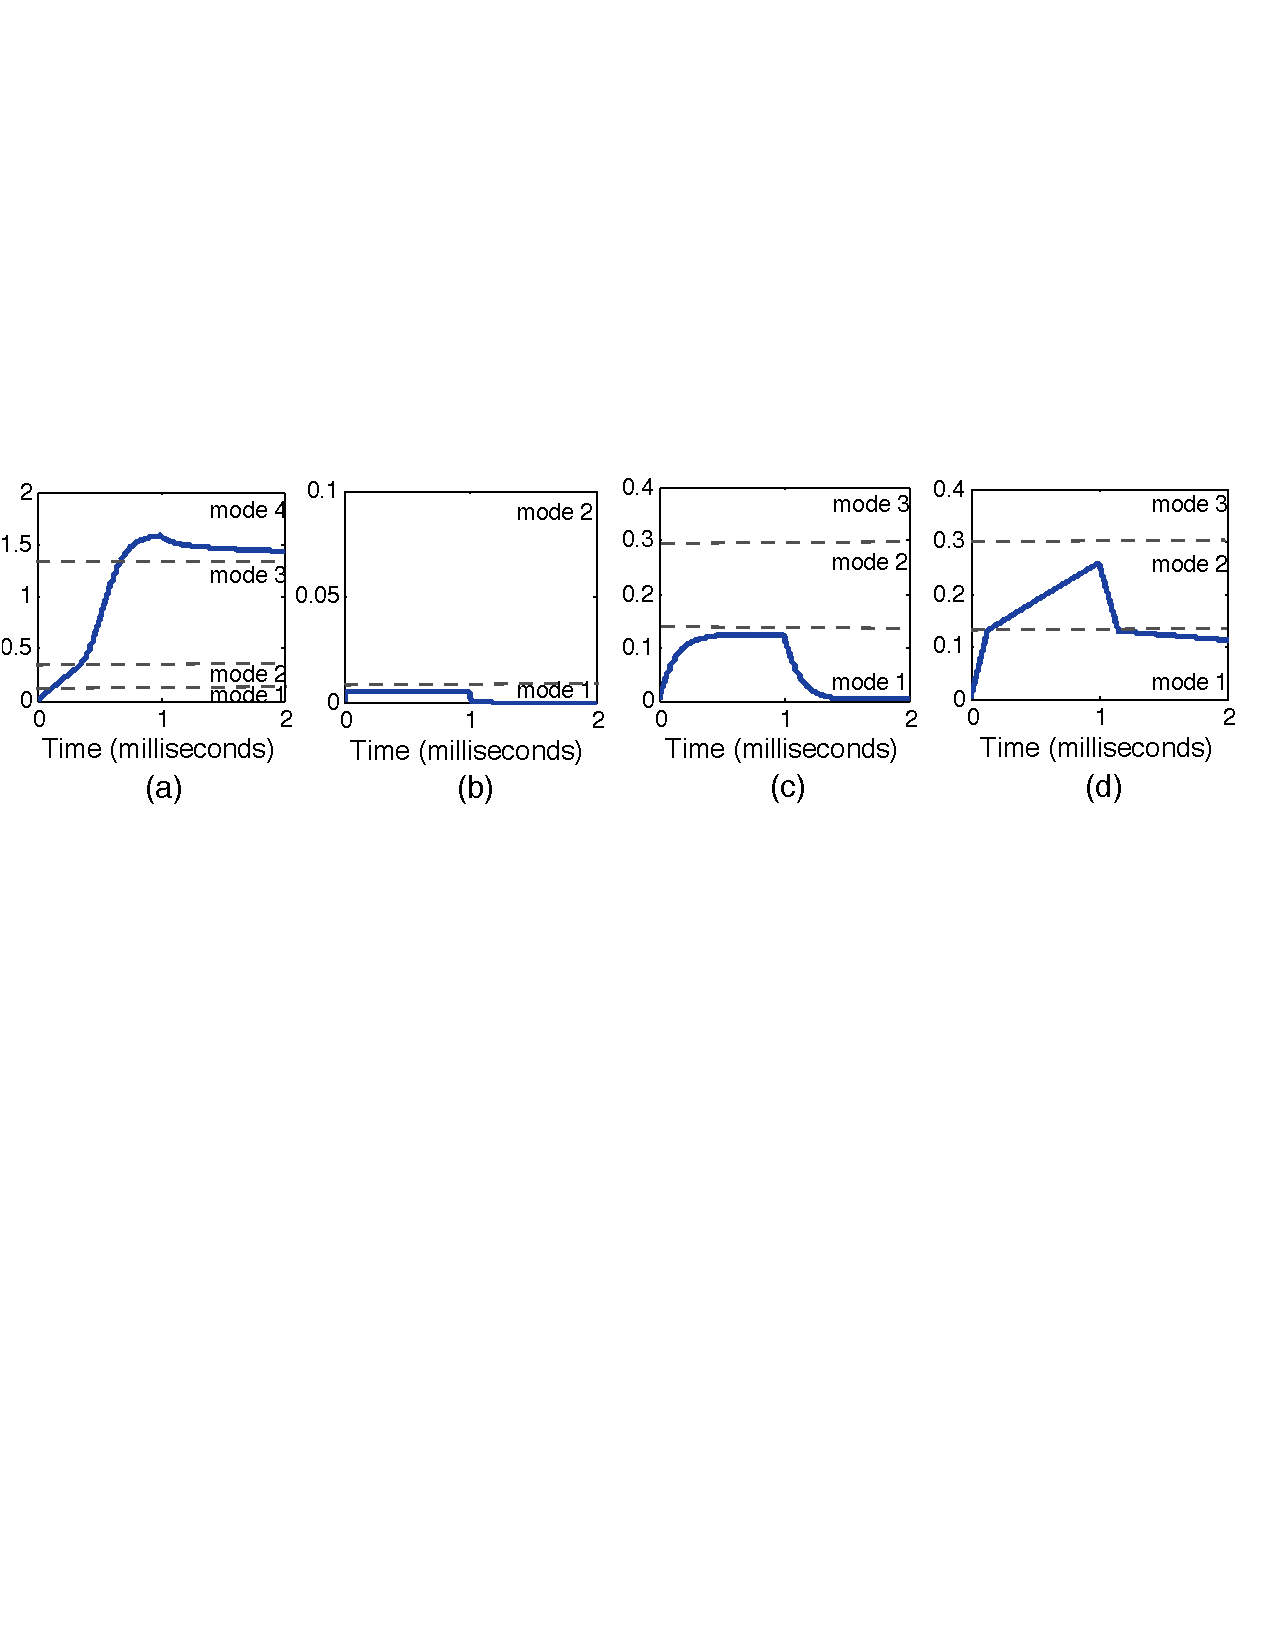
\includegraphics[scale=0.6]{fig-cardiactraj2}
\caption{Simulation results using disease related parameter values. (a) Original parameters (b) $\tau_{o1}=0.0055$ (c) $\tau_{o2} = 0.125$ (d) $\tau_{so1} =1.2$, $\tau_{so2} =1.0$ }
\label{cresults}
 %\vspace{-0.7cm}
\end{figure}

%%% Local Variables:
%%% TeX-master: "main"
%%% End:

\section{Conclusion}
%Hybrid automata are well-studied formalisms for modeling the behavior of biological systems. In this article, we have presented a framework using $\delta$-complete decision procedures for the parameter identification of hybrid biological systems. We have used $\delta$-satisfiable formulas to describe parameterized hybrid automata and to encode parameter synthesis problems. We have employed the $\delta$-decision procedures to perform bounded model checking, and developed an interval constrains propagation based algorithm to obtain the resulting parameters.
We have presented a framework using $\delta$-complete decision procedures for the parameter identification 
of hybrid biological systems. We have used $\delta$-satisfiable formulas to describe parameterized hybrid automata 
and to encode parameter synthesis problems. We have employed $\delta$-decision procedures to perform bounded model 
checking, and developed an algorithm to obtain the resulting parameters.
We have demonstrated the applicability of our method on a highly nonlinear hybrid model of a cardiac cell that cannot
be handled by other verification tools. We have successfully ruled out model candidates which did not fit 
experimental observations, and we have identified critical parameter ranges that can induce cardiac disorders.
Our method has the potential to be applied to model classes such as hybrid functional Petri nets models \citep{hfpn}. 
We plan to explore this in future work. Another interesting direction is applying our method for parameter estimation 
from experimental data. By properly encoding the noisy wet-lab experimental data using logic formulas, bounded model 
checking can be utilized to find the unknown parameter values. In this respect, the parameter 
estimation framework presented in \cite{liu13} promises to offer helpful pointers.

%Finally, we will develop a GPU-based implementation of our method to exploit the inherent massive parallelism in generating trajectories through numerical integration.





%\paragraph{Funding:} This work has been partially supported by the National Science Foundation (NSF), NSF Expeditions in Computing.

%\paragraph{Conflict of Interest:} none declared.


%%% Local Variables:
%%% TeX-master: "main"
%%% End:





%ACKNOWLEDGMENTS are optional
%\section{Acknowledgments}



\bibliographystyle{abbrv}
\bibliography{sigproc}

%\newpage
\section*{Appendix: $\lrf$-Formulas and $\delta$-Decidability}

We will use a logical language over the real numbers that allows arbitrary {\em computable real functions}~\cite{CAbook}. We write $\lrf$ to represent this language. Intuitively, a real function is computable if it can be numerically simulated up to an arbitrary precision. For the purpose of this paper, it suffices to know that almost all the functions that are needed in describing hybrid systems are Type 2 computable, such as polynomials, exponentiation, logarithm, trigonometric functions, and solution functions of Lipschitz-continuous ordinary differential equations.

More formally, $\lrf = \langle \mathcal{F}, > \rangle$ represents the first-order signature over the reals with the set $\mathcal{F}$ of computable real functions, which contains all the functions mentioned above. Note that constants are included as 0-ary functions. $\lrf$-formulas are evaluated in the standard way over the structure $\mathbb{R}_{\mathcal{F}}= \langle \mathbb{R}, \mathcal{F}^{\mathbb{R}}, >^{\mathbb{R}}\rangle$. It is not hard to see that  we can put any $\lrf$-formula in a normal form, such that its atomic formulas are of the form $t(x_1,...,x_n)>0$ or $t(x_1,...,x_n)\geq 0$, with $t(x_1,...,x_n)$ composed of functions in $\mathcal{F}$. To avoid extra preprocessing of formulas, we can explicitly define $\mathcal{L}_{\mathcal{F}}$-formulas as follows.
\begin{definition}[$\lrf$-Formulas]
Let $\mathcal{F}$ be a collection of computable real functions. We define:
\begin{align*}
t& := x \; | \; f(t(\vec x)), \mbox{ where }f\in \mathcal{F} \mbox{ (constants are 0-ary functions)};\\
\varphi& := t(\vec x)> 0 \; | \; t(\vec x)\geq 0 \; | \; \varphi\wedge\varphi
\; | \; \varphi\vee\varphi \; | \; \exists x_i\varphi \; |\; \forall x_i\varphi.
\end{align*}
In this setting $\neg\varphi$ is regarded as an inductively defined operation
which replaces atomic formulas $t>0$ with $-t\geq 0$, atomic formulas $t\geq 0$
with $-t>0$, switches $\wedge$ and $\vee$, and switches $\forall$ and $\exists$.
\end{definition}
\begin{definition}[Bounded $\lrf$-Sentences]
We define the bounded quantifiers $\exists^{[u,v]}$ and $\forall^{[u,v]}$ as
$\exists^{[u,v]}x.\varphi =_{df}\exists x. ( u \leq x \land x \leq v \wedge
\varphi)$ and $
\forall^{[u,v]}x.\varphi =_{df} \forall x. ( (u \leq x \land x \leq v)
\rightarrow \varphi)$
where $u$ and $v$ denote $\lrf$ terms, whose variables only
contain free variables in $\varphi$ excluding $x$. A {\em bounded $\lrf$-sentence} is
$$Q_1^{[u_1,v_1]}x_1\cdots Q_n^{[u_n,v_n]}x_n\;\psi(x_1,...,x_n),$$
where $Q_i^{[u_i,v_i]}$ are bounded quantifiers, and $\psi(x_1,...,x_n)$ is
quantifier-free.
\end{definition}
\begin{definition}[$\delta$-Variants]\label{variants}
Let $\delta\in \mathbb{Q}^+\cup\{0\}$, and $\varphi$ an
$\lrf$-formula
$$\varphi: \ Q_1^{I_1}x_1\cdots Q_n^{I_n}x_n\;\psi[t_i(\vec x, \vec y)>0;
t_j(\vec x, \vec
y)\geq 0],$$ where $i\in\{1,...k\}$ and $j\in\{k+1,...,m\}$. The {\em
$\delta$-weakening} $\varphi^{\delta}$ of $\varphi$ is
defined as the result of replacing each atom $t_i > 0$ by $t_i >
-\delta$ and $t_j \geq 0$ by $t_j \geq -\delta$:
$$\varphi^{\delta}:\ Q_1^{I_1}x_1\cdots Q_n^{I_n}x_n\;\psi[t_i(\vec x, \vec
y)>-\delta; t_j(\vec x,
\vec y)\geq -\delta].$$
It is clear that $\varphi\rightarrow\varphi^{\delta}$~(see \cite{gao12b}).
\end{definition}
In~\cite{dreal}, we have proved that the following $\delta$-decision problem is decidable, which is the basis of our framework.
\begin{theorem}[$\delta$-Decidability]\label{delta-decide} Let $\delta\in\mathbb{Q}^+$ be
arbitrary. There is an algorithm which, given any bounded $\lrf$-sentence $\varphi$,
correctly returns one of the following two answers:
\begin{itemize}
\item $\delta$-$\mathsf{True}$: $\varphi^{\delta}$ is true.
\item $\mathsf{False}$: $\varphi$ is false.
\end{itemize}
When the two cases overlap, either answer is correct.
\end{theorem}
\begin{theorem}[Complexity]\label{compmain}
Let $S$ be a class of $\lrf$-sentences, such that for any $\varphi$ in $S$, the terms in $\varphi$ are in Type 2 complexity class $\mathsf{C}$. Then, for any $\delta\in \mathbb{Q}^+$, the $\delta$-decision problem for bounded $\Sigma_n$-sentences in $S$ is in $\mathsf{(\Sigma_n^P)^C}$.
\end{theorem}


\section*{Appendix: BCF Model in dReach}

\begin{verbatim}
//Translated to drh by Sicun Gao on Apr-18-2013
// ===============================================================
// ==   Minimal Resistor Model (4 state variables)              ==
// ==                                                           ==
// ==   Author:  E. Bartocci                                    ==
// ==                                                           ==
// ==   Date:  11/05/10                                         ==
// ==                                                           ==
// ==   Free distribution with authors permission               ==
// ==                                                           ==
// ==   SUNY Stony Brook, Stony Brook, NY                       ==
// ==                                                           ==
// ===============================================================
// The following are the parameters that you can find in the paper
// A. Bueno-Orovio, M. Cherry, and F. Fenton, `Minimal model for
// human ventricular action potentials in tissue', Journal of
// Theoretical Biology, no. 253, pp. 544?560, 2008.
// ===============================================================

#define  EPI_TVP         1.4506
#define  EPI_TV1M       60.0
#define  EPI_TV2M     1150.0
#define  EPI_TWP       200.0
#define  EPI_TW1M       60.0
#define  EPI_TW2M       15.0

#define  EPI_TS1        2.7342
#define  EPI_TS2       16.0     //The same with Flavio's paper
#define  EPI_TFI        0.11    //The same with Flavio's paper

#define  EPI_TO1      400    //The same with Flavio's paper
#define  EPI_TO2        6.0      //The same with Flavio's paper
#define  EPI_TSO1      30.0181 //The same with Flavio's paper
#define  EPI_TSO2       0.9957  //The same with Flavio's paper

#define  EPI_TSI        1.8875  // We have TSI1 and TSI2 TSI in Flavio's paper


#define  EPI_TWINF      0.07    //The same with Flavio's paper
#define  EPI_THV        0.3     //EPUM The same of Flavio's paper
#define  EPI_THVM       0.006   //EPUQ The same of Flavio's paper
#define  EPI_THVINF     0.006   //EPUQ The same of Flavio's paper
#define  EPI_THW        0.13    //EPUP The same of Flavio's paper
#define  EPI_THWINF     0.006   //EPURR In Flavio's paper 0.13
#define  EPI_THSO       0.13    //EPUP The same of Flavio's paper
#define  EPI_THSI       0.13    //EPUP The same of Flavio's paper
#define  EPI_THO        0.006   //EPURR The same of Flavio's paper

#define  EPI_KWM       65.0     //The same of Flavio's paper
#define  EPI_KS         2.0994  //The same of Flavio's paper
#define  EPI_KSO        2.0458  //The same of Flavio's paper

#define  EPI_UWM        0.03    //The same of Flavio's paper
#define  EPI_US         0.9087  //The same of Flavio's paper
#define  EPI_UO         0.0     //The same of Flavio's paper
#define  EPI_UU         1.55    //The same of Flavio's paper
#define  EPI_USO        0.65    //The same of Flavio's paper

#define  jfi1  0.0
#define  jso1  (u/EPI_TO1)
#define  jsi1  0.0

#define  jfi2  0.0
#define  jso2  (u/EPI_TO2)
#define  jsi2  0.0


#define  jfi3  0.0
#define  jso3  1.0/(EPI_TSO1+((EPI_TSO2- EPI_TSO1)*(1/(1+exp(-2*EPI_KSO*(u- EPI_USO))))))
#define  jsi3  (0 - (w * s)/EPI_TSI)

#define  jfi4  (0 - v * (u - EPI_THV) * (EPI_UU - u)/EPI_TFI)
#define  jso4  (1.0 / (EPI_TSO1+((EPI_TSO2 - EPI_TSO1)*(1/(1+exp(-2*EPI_KSO*(u- EPI_USO)))))))
#define  jsi4  ( 0 - (w * s)/EPI_TSI)
#define	 stim  1.0 // The external stimulation is a rectangular pulse of 
                      height 1 and length 1ms. Since u reach its maximum 
                      during the stimulation, time scale is set to be [0,1] 
[0, 2.0] u;
[0, 2.0] v;
[0, 2.0] w;
[0, 2.0] s;
[0, 1] tau;
[0, 1] time;

{mode 1;

invt:    (u >= 0);
         (u <= 0.006);
         (v >= 0);
         (w >= 0);
         (s >= 0);
         (tau >= 0);
flow:
         d/dt[tau] = 1.0;
         d/dt[u] = (stim - jfi1) - (jso1 + jsi1);
         d/dt[w] = ((1.0 -(u/EPI_TWINF) - w)/(EPI_TW1M + (EPI_TW2M - EPI_TW1M) * 
                   (1/(1+exp(-2*EPI_KWM*(u - EPI_UWM))))));
         d/dt[v] = ((1.0 - v)/EPI_TV1M);
         d/dt[s] = (((1/(1+exp( -2 * EPI_KS * (u - EPI_US) ))) - s)/EPI_TS1);
jump:
         (u >= 0.006) ==> @2 (and (tau' = tau) (u' = u) (v'= v) (w' = w) (s' = s));
}

{mode 2;

invt:
         (u >= 0.006);
         (u <= 0.13);
         (v >= 0);
         (w >= 0);
         (s >= 0);
         (tau >= 0);
flow:
         d/dt[tau] = 1.0;
         d/dt[u] = (stim - jfi2) - (jso2 + jsi2);
         d/dt[w] = ((0.94-w)/(EPI_TW1M + (EPI_TW2M - EPI_TW1M) * 
                   (1/(1+exp(-2*EPI_KWM*(u - EPI_UWM))))));
         d/dt[v] = (-v/EPI_TV2M);
         d/dt[s] = (((1/(1+exp( -2 * EPI_KS * (u - EPI_US) ))) - s)/EPI_TS1);
jump:
         (u >= 0.13) ==> @3 (and (tau' = tau) (u' = u) (v'= v) (w' = w) (s' = s));
}

{mode 3;

invt:
         (u >= 0.13);
         (u <= 0.3);
         (v >= 0);
         (w >= 0);
         (s >= 0);
         (tau >= 0);
flow:
         d/dt[tau] = 1.0;
         d/dt[u] = (stim - jfi3) - (jso3 + jsi3);
         d/dt[w] = (-w/EPI_TWP);
         d/dt[v] = (-v/EPI_TV2M);
         d/dt[s] = (((1/(1+exp( -2 * EPI_KS * (u - EPI_US) ))) - s)/EPI_TS2);
jump:
         ( u >= 0.3) ==> @4 (and (tau' = tau) (u' = u) (v'= v) (w' = w) (s' = s));
}

{mode 4;

invt:
         (u >= 0.3);
         (v >= 0);
         (w >= 0);
         (s >= 0);
         (tau >= 0);
flow:
         d/dt[tau] = 1.0;
         d/dt[u] =  (stim - jfi4) - (jso4 + jsi4);
         d/dt[w]  = (-w/EPI_TWP);
         d/dt[v]  = (-v/EPI_TVP);
         d/dt[s]  = (((1/(1+exp( -2 * EPI_KS * (u - EPI_US) ))) - s)/EPI_TS2) ;
jump:
         (u > 2.0) ==> @4 (and (tau' = tau) (u' = u) (v'= v) (w' = w) (s' = s));
}

init:  @1 (and (tau = 0) (u = 0.0) (v = 1.0) (w = 1.0) (s = 0.0));

goal:  @4 (and (tau = 1) (u >= 0.3) (u <= 2) (v >= 0) (v <= 2) 
          (w >= 0) (w <= 2) (s >= 0) (s <= 2));
\end{verbatim}



\end{document}
